\chapter{Mandelbrot percolation - methods and results}
\label{ch:mandelbrot_experimental}

\section{Introduction}

Now we turn our attention to the so called Mandelbrot percolation, which is also known in the literature as Fractal percolation. The idea is, again, to study the clusters structure and distribution, but the coloring of the lattice happens in a different way: instead of doing a single pass over the lattice and coloring the nodes at random, we do this process repeatedly - at each step, we subdivide each node in the lattice into a number of "sub-nodes" and color the remaining "alive" (not yet colored) nodes with probability $p$. An illustration of this process can be seen in \autoref{fig:mandelbrot_process}. 
Each iteration generates a lattice $A_n$ (which is, of course, highly correlated with the previous lattice $A_{n-1}$). Mandelbrot percolation is the study of the limit of this process the number of steps increases arbitrarily, that, is $\lim_{n\to\infty} A_n$.

\begin{figure}[H]
  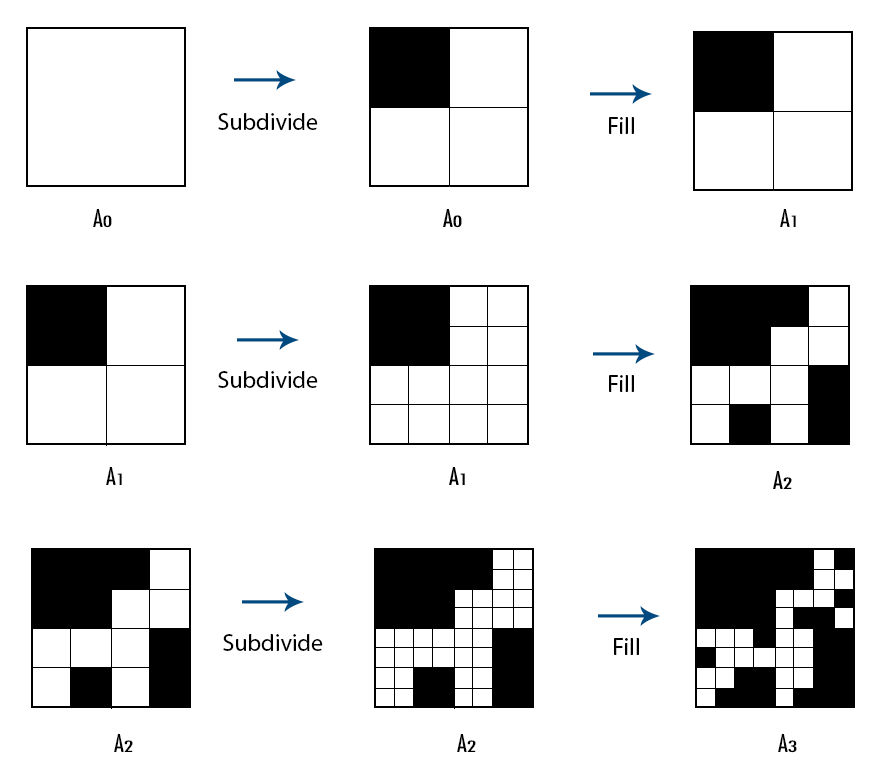
\includegraphics[width=\linewidth]{Images/mandelbrot_process.png}
  \caption{Illustration of the Mandelbrot percolation iteration process, showing three iterations}
  \label{fig:mandelbrot_process}
\end{figure}


\begin{figure}[H]
  \includegraphics[width=\linewidth]{Images/mandelbrot_lattice.png}
  \caption{A Mandelbrot percolation lattice after 11 iterations}
  \label{fig:mandelbrot_lattice}
\end{figure}


\section{Simulation methods}

The simulations were run, again, on a 2D periodic square lattice. 
We studied three properties: the percolation probability, mean cluster size and percolating cluster strength. We explicitly used exactly the same definitions, methods and algorithms as for the 2D case - the reason for this is that this way, a direct comparison is possible. The precise description of these methods is available in \autoref{ch:classical_experimental}.

\section{Percolation probability}

In \autoref{fig:simm_perc_prob_2}, the first thing we notice is that the the critical probability $p_c$ is much lower than in the classical percolation model - at first sight, it's clear that $p_c < 0.3$. The reason for this is somewhat obvious. For a given $(p, L)$ pair, in classical percolation, we do a single pass over the lattice, whereas in the Mandelbrot model, we have done several passes previously, when the lattice was smaller. So on top of making multiple passes, the previous passes happened when each node represented a bigger part fraction of the lattice.

\begin{figure}[H]
  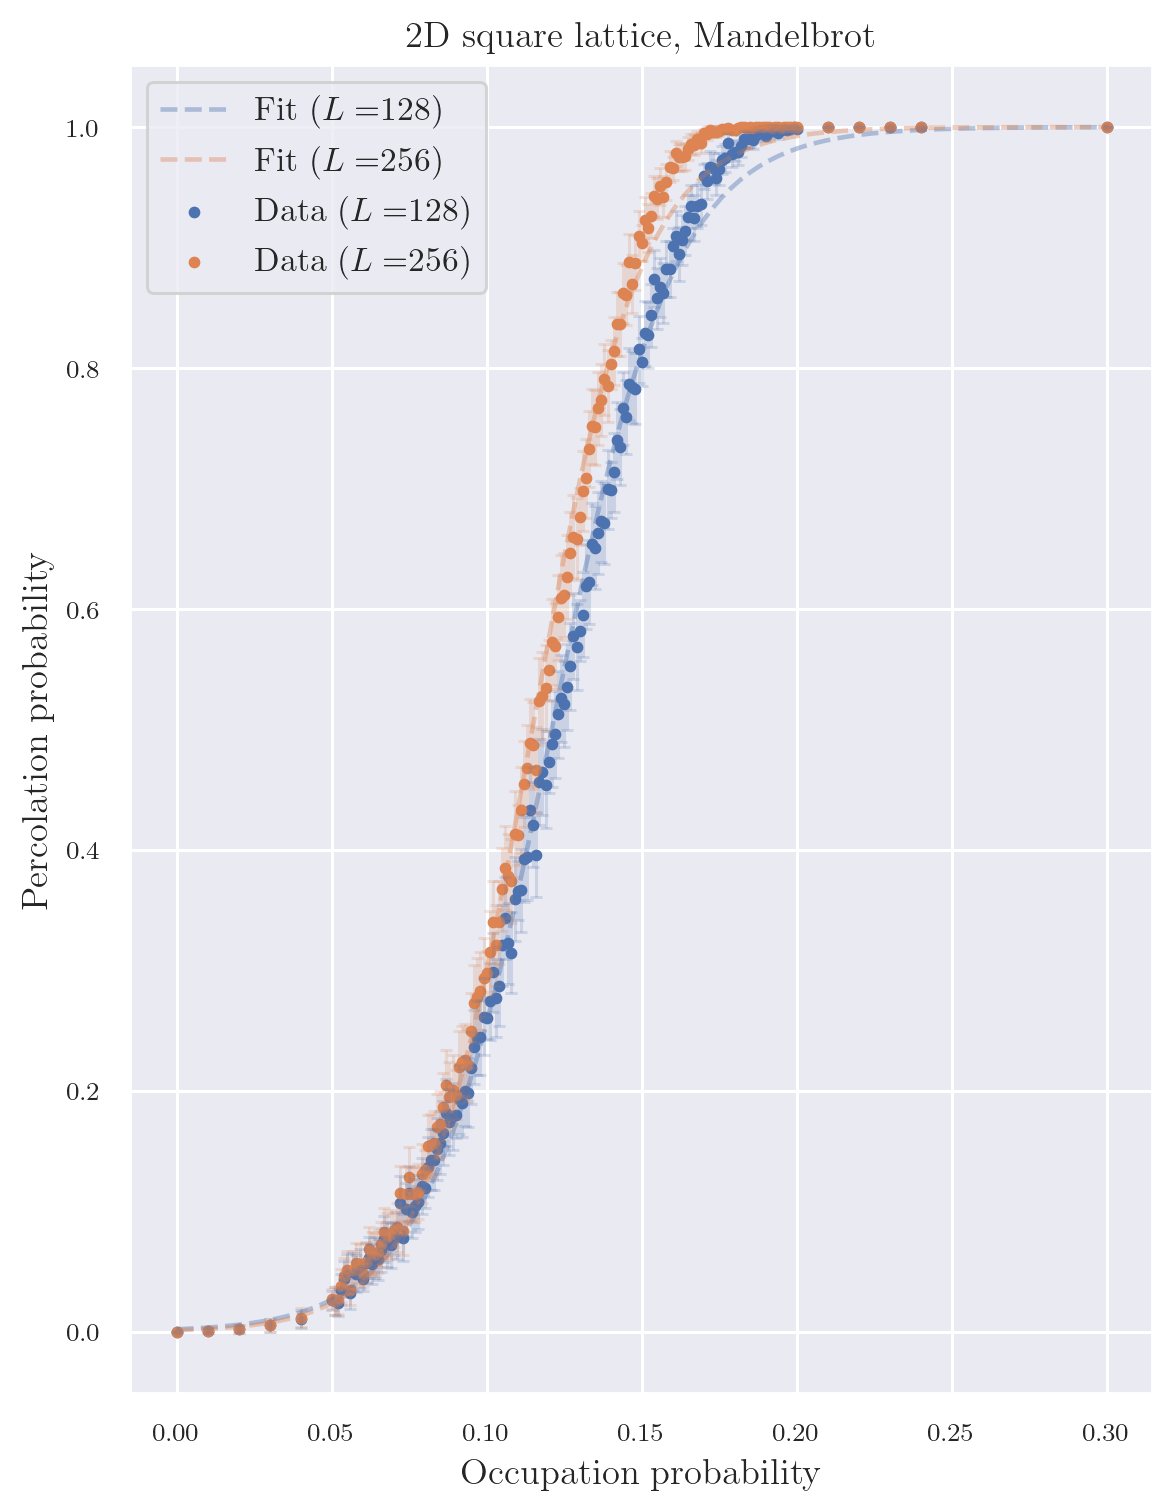
\includegraphics[width=\linewidth]{Images/simm_perc_prob_2.png}
  \caption{Percolation probability in the Mandelbrot percolation model}
  \label{fig:simm_perc_prob_2}
\end{figure}

Just like in classical percolation, we fitted a hyperbolic tangent function to the data, and for $L=256$, which is the largest size we simulated for the Mandelbrot model, we find that the the percolation probability reaches the $0.5$ mark when $p=\textbf{0.1273} \pm 0.021$. We point out that the fit is noticeably worse for the Mandelbrot model than in the case of classical percolation, which suggests an underlying fundamental difference between the models. Additionally, we notice that plots obtained for $L=128$ and $L=256$ are in relation to each other in a different way than the equivalent curves in the classical percolation case. In comparison with \autoref{fig:sim_perc_prob_2}, for example, one notices that whereas there, the curves have a sharp increase at very different occupation probabilities, here they are much closer to each other for low values of $p$, and remain much closer. We hypothesize that this happens, again, because the lattices are much more closely related here - the additional pass used in the $L=256$ happens at a smaller length scale and therefore has a less pronounced effect on the curve.

The errors were computed using the same method as described in \autoref{sec:sim_perc_prob}.

\section{Percolating cluster strength}

The percolation cluster strength results for the Mandelbrot percolation simulations can be seen in \autoref{fig:simm_perc_clust_strength_1}. The curve looks qualitatively pretty similar to the one we had for classical percolation (see \autoref{fig:sim_perc_clust_strength_1}).


\begin{figure}[H]
  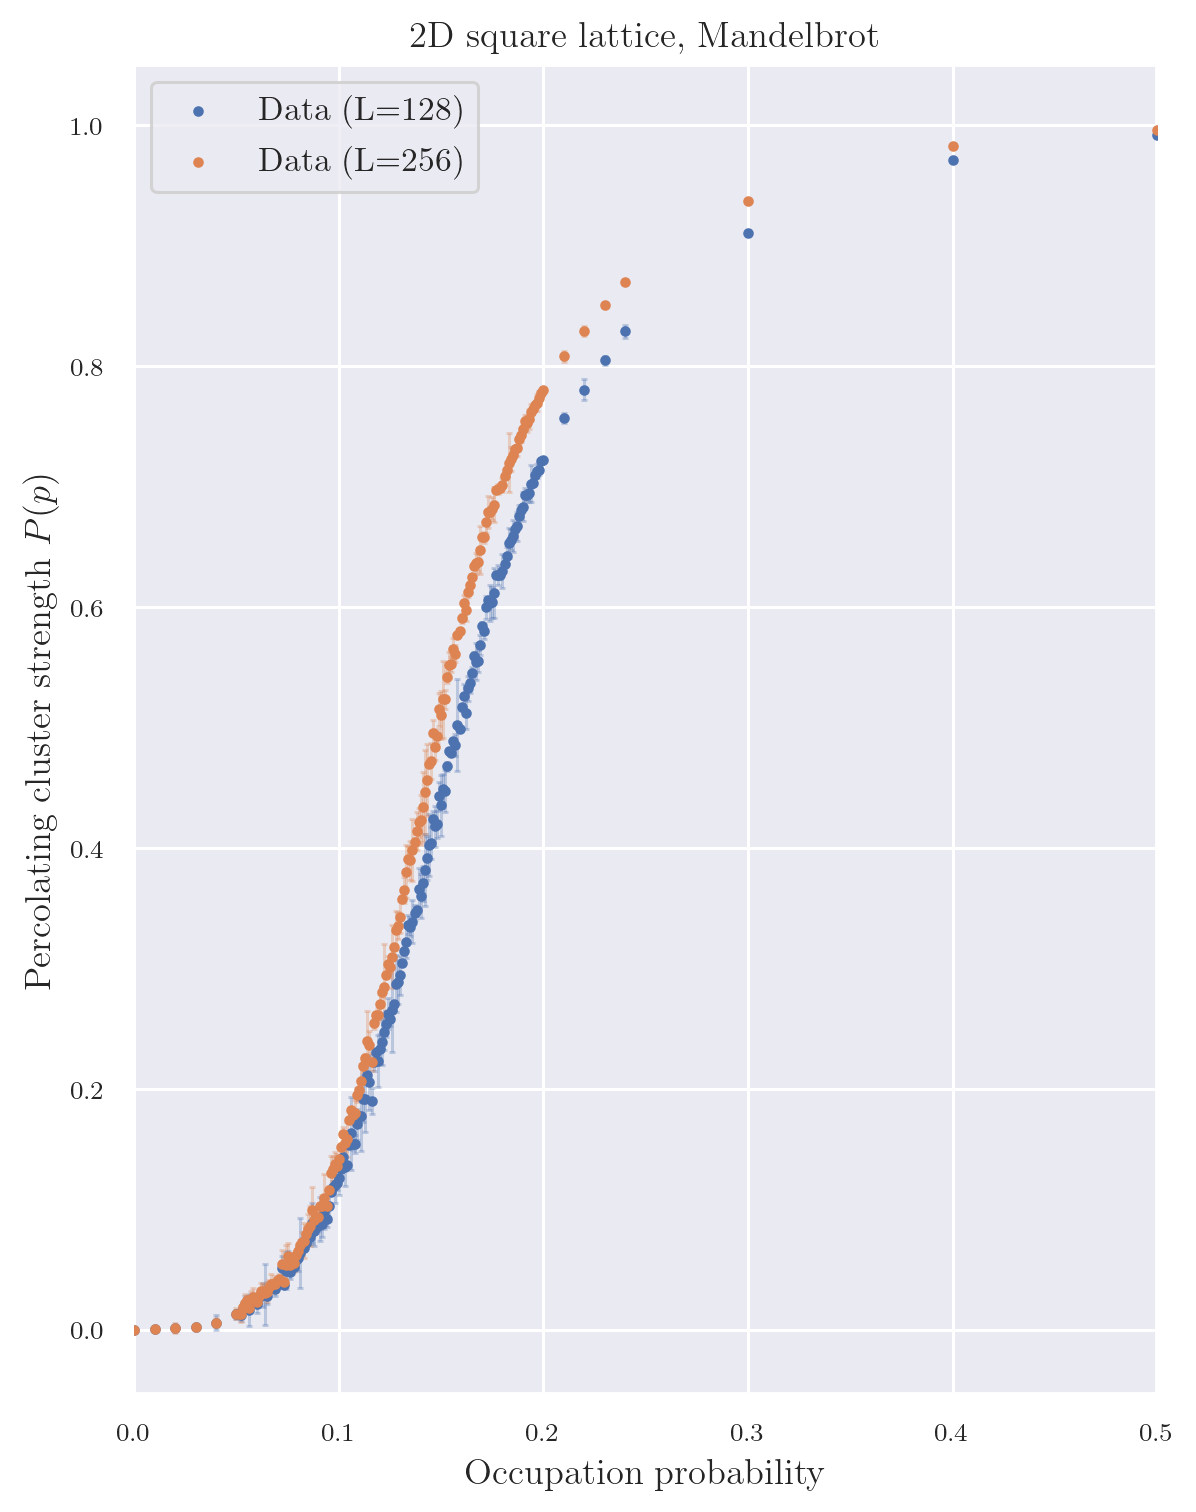
\includegraphics[width=\linewidth]{Images/simm_perc_clust_strength_1.png}
  \caption{Percolating cluster strength for the Mandelbrot percolation model}
  \label{fig:simm_perc_clust_strength_1}
\end{figure}

Other than the lower values for the critical occupation probability discussed above, another interesting fact worth pointing out is that although for both models the curve becomes essentially a linear function towards higher values of the occupation probability $p$, the slope of the curve is noticeably smaller for the Mandelbrot case. The reason for this is not immediately obvious and warrants further investigation.
The errors were computed using the same method as described in \autoref{sec:sim_perc_clust_strength}.


\section{Mean cluster size}

The results for the mean cluster size can be seen in \autoref{fig:simm_mean_cluster_size_1}. 

\begin{figure}[H]
  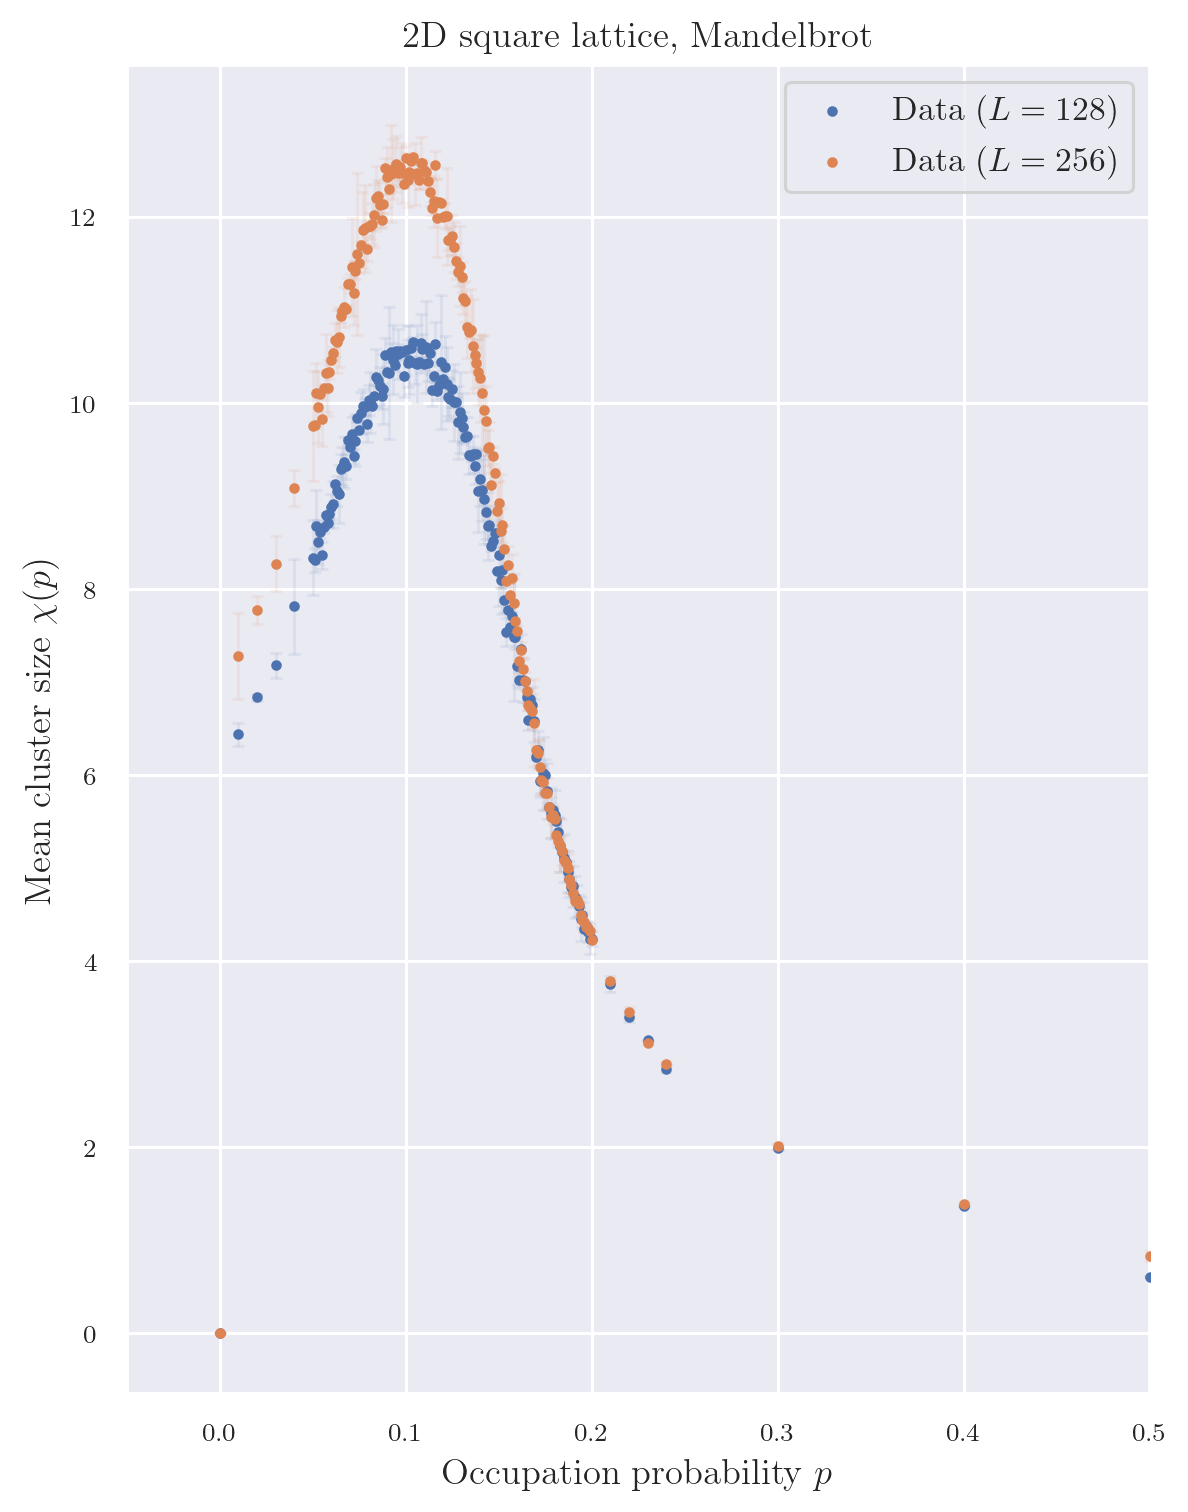
\includegraphics[width=\linewidth]{Images/simm_mean_cluster_size_1.png}
  \caption{Mean cluster size in the Mandelbrot percolation model}
  \label{fig:simm_mean_cluster_size_1}
\end{figure}

In comparison with the classical percolation plots (see \autoref{fig:sim_mean_cluster_size_1}), it is curious that the peak heights are smaller for the Mandelbrot percolation. The reason for this is, again not immediately obvious - the reader is invited to investigate this further.
The errors were computed using the same method as described in \autoref{sec:sim_mean_clust_size}.

\section{Conclusion}

Even in the case of classical percolation, which has been widely studied by many people in the last 50 years, we hope that this work provides a solid numerical and computation basis upon which further investigation can be made. We provide both the data used in these analysis and the code used to generate it in hopes of facilitating collaboration and reuse, as well as inspiring a more modern approach to computational research in general. 

For the case of Mandelbrot percolation, this work is intended as a first step towards computational analysis of the model, in particular emphasizing differences and similarities as compared to the classical percolation models. While we didn't intend to provide a through and careful theoretical justification of the results obtained, this is encouraged for the curious reader. 

The author is happy to answer any questions - feel free to email \url{alansammarone@gmail.com}.
